%iffalse
\let\negmedspace\undefined
\let\negthickspace\undefined
\documentclass[journal,12pt,onecolumn]{IEEEtran}
\usepackage{cite}
\usepackage{amsmath,amssymb,amsfonts,amsthm}
\usepackage{algorithmic}
\usepackage{multicol}
\usepackage{graphicx}
\usepackage{textcomp}
\usepackage{xcolor}
\usepackage{txfonts}
\usepackage{listings}
\usepackage{enumitem}
\usepackage{mathtools}
\usepackage{gensymb}
\usepackage{comment}
\usepackage[breaklinks=true]{hyperref}
\usepackage{tkz-euclide} 
\usepackage{listings}
\usepackage{gvv}                                        
%\def\inputGnumericTable{}                                 
\usepackage[latin1]{inputenc}                                
\usepackage{color}                                            
\usepackage{array}                                            
\usepackage{longtable}                                       
\usepackage{calc}                                             
\usepackage{multirow}                                         
\usepackage{hhline}                                           
\usepackage{ifthen}                                           
\usepackage{lscape}
\usepackage{tabularx}
\usepackage{array}
\usepackage{float}
\newtheorem{theorem}{Theorem}[section]
\newtheorem{problem}{Problem}
\newtheorem{proposition}{Proposition}[section]
\newtheorem{lemma}{Lemma}[section]
\newtheorem{corollary}[theorem]{Corollary}
\newtheorem{example}{Example}[section]
\newtheorem{definition}[problem]{Definition}
\newcommand{\BEQA}{\begin{eqnarray}}
\newcommand{\EEQA}{\end{eqnarray}}
\newcommand{\define}{\stackrel{\triangle}{=}}
\theoremstyle{remark}
\newtheorem{rem}{Remark}

% Marks the beginning of the document
\begin{document}
\bibliographystyle{IEEEtran}
\vspace{3cm}

\title{\textbf{NCERT 10.4.EX1}}
\author{EE24BTECH11032- John Bobby}
\maketitle
\bigskip
\textbf{Alex and Sam together have 45 marbles. Both of them lost 5 marbles each, and the product of the number of marbles they have is 124. Find how many marbles they had at the beginning.}
\textbf{Solution:}\\
Let  the number of marbles Alex have at the beginning$=x$\\
The number of marbles Sam have $=45-x$\\
After losing $5$ marbles,\\
Number of marbles alex has $x-5$\\
Sam now has $45-x-5=50-x$\\
Product of marbles $=124$\\
$\brak{x-5}\brak{50-x}=124$\\
On rearranging,\\
$x^2-45x+324=0$
\section{Quadratic Formula}
Consider an equation, 
	\begin{align}
		ax^2 + bx + c &= 0 \\
	        x^2 + \frac{b}{a} x + \frac{c}{a} &= 0 \label{eq:qe} \\
		x^2 + 2 \frac{b}{2a} x + \frac{b^2}{4a^2} - \frac{b^2}{4a^2} + \frac{c}{a} &= 0 \\
		\brak{x + \frac{b}{2a}}^2 + \brak{\frac{4ac - b^2}{4a^2}} &= 0 \\
		\brak{x + \frac{b}{2a}} &= \frac{\sqrt{b^2 - 4ac}}{2a} \\
		x &= \frac{-b \pm \sqrt{b^2 - 4ac}}{2a}
	\end{align}
	which is the quadratic formula. \\
For the quadratic equation $x^2-45x+324=0$,\\
$a=1,b=-45,c=324$\\
On solving we get the roots to be $x=9$ and $x=36$

\section{Eigen Values-Method}
Consider the equation, \eqref{eq:qe}. It can be rearranged as
	\begin{align}
		\lambda ^2 + \frac{b}{a} \lambda + \frac{c}{a} &= 0 \\
		\lambda \brak{\lambda + \frac{b}{a}} + \frac{c}{a} &= 0 \\
		-\lambda \brak{-\lambda - \frac{b}{a}} - (-1) \frac{c}{a} &= 0
	\end{align}
	This can be considered equivalent to the determinant of the matrix, 
	\begin{align}
		\myvec{-\lambda & 1 \\ -\frac{c}{a} & \frac{-b}{a} - \lambda} \label{eq:matrix}
	\end{align}
	Clearly, it can be seen that the eigenvalues of the matrix 
	\begin{align}
		\myvec{0 & 1 \\ \frac{-c}{a} & \frac{-b}{a}} \label{eq:cmat}
	\end{align}
	are the roots of the required quadratic equation. This matrix, \eqref{eq:cmat} is called the \textbf{Companion matrix} \brak{\vec{C}}. \\
	For the given question, 
	\begin{align}
		\vec{C} &= \myvec{0 & 1 \\ -2 & 3}
	\end{align}
	\textbf{QR ALGORITHM} :
	Eigenvalues of the companion matrix can be found using QR algorithm. Using the Gram-Schmidt orthogonalization, the matrix $\vec{C}$ can be factorized into
	\begin{align}
		\vec{C} &= \vec{Q} \vec{R}
	\end{align}
	where, 
	\begin{align}
		\vec{Q} &= Orthonormal matrix \\
		\vec{R} &= Upper triangular matrix
	\end{align}
	This process can be continues as
	\begin{align}
		\vec{C_{k}} &= \vec{Q_{k}} \vec{R_{k}} \\
		\vec{C_{k+1}} &= \vec{R_{k}} \vec{Q_{k}}
	\end{align}
	As $k \to \infty$, the diagonal elements of $\vec{Q_{k}}$ converge to the eigenvalues of the matrix.
	It can be seen that eigenvalues are 1 and 2.
	\textbf{Newton-Raphson method} : \\
		We have, 
		\begin{align}
			x_{n+1} &= x_{n} - \frac{f(x_{n})}{f^{\prime}(x_{n})}	\\
			x_{n+1} &= x_{n} - \frac{x_{n}^2 - 45x_{n} + 324}{2 x_{n} - 45}
		\end{align}
		Iterating and updating the value of $x_{n}$, we can obtain the roots of the quadratic equation. \\
		The roots found using this method taking the initial guesses as 5 and 25 are 9 and 36
 respectively.
\begin{figure}[h]
\centering
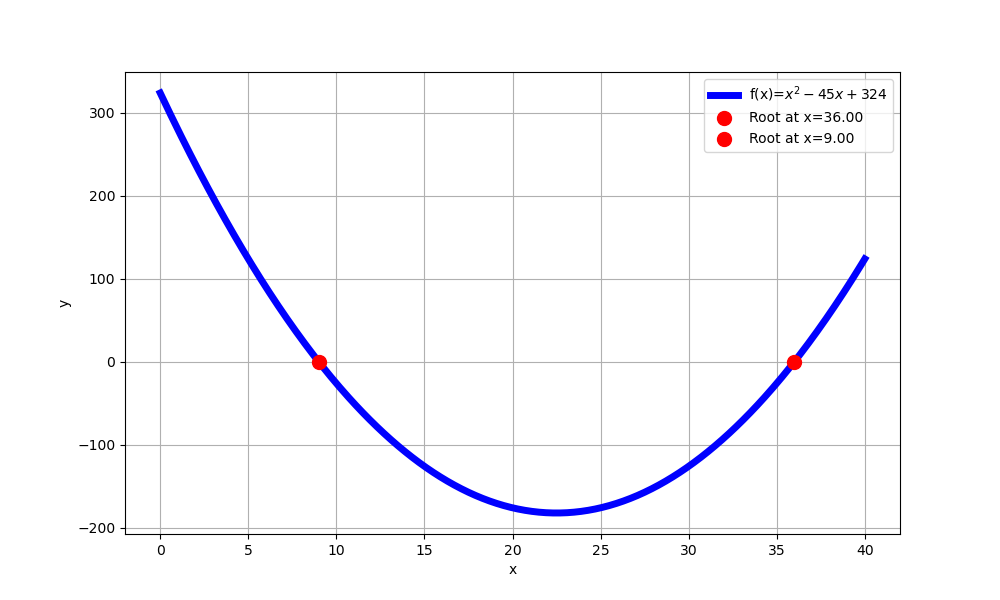
\includegraphics[width=\columnwidth]{figs/Q5.png}
\caption{Plot using Newton-Raphson method}
\label{fig:Plot1} 
\end{figure}
\end{document}

 
 








\end{document}
